\documentclass[9pt]{book}
%\usepackage[spanish]{babel}
\usepackage{fancyhdr}
\usepackage{color}
\usepackage[latin1]{inputenc}
\usepackage{indentfirst}
\usepackage{graphicx}
\usepackage{graphicx}
\graphicspath{ {./imagenes/} }
%\usepackage{rotating}
\usepackage{amssymb}
\usepackage{amsmath}
\usepackage{gensymb}
\usepackage{url}
\usepackage{xcolor}
\usepackage{listings}
%\usepackage{shapepar}
%\usepackage[small]{caption}
%\usepackage{lscape}
%\usepackage{natbib}
\pagestyle{fancy}
\definecolor{mGreen}{rgb}{0,0.6,0}
\definecolor{mGray}{rgb}{0.5,0.5,0.5}
\definecolor{mPurple}{rgb}{0.58,0,0.82}
\definecolor{backgroundColour}{rgb}{0.95,0.95,0.92}
%\usepackage{mathrsfs}
%\usepackage{multirow}
\newcommand{\ihat}{\mathbf {\hat \imath}}
\newcommand{\jhat}{\mathbf {\hat \jmath}}


%\renewcommand{\chaptermark}[1]{\markboth{#1}{}}
%\renewcommand{\sectionmark}[1]{\markright{\thesection\ #1}}
%\lhead[\fancyplain{}{\bfseries\thepage}] {\fancyplain{}{\bfseries\rightmark}}
%\rhead[\fancyplain{}{\bfseries\leftmark}] {\fancyplain{}{\bfseries\thepage}}
%\cfoot{}
%\newcommand{\ud}{\;\mathrm{d}}
%\renewcommand{\sin}{\mbox{\,sen\,}}
%\renewcommand{\tablename}{Tabla}
%\setlength{\captionmargin}{19pt}
%\renewcommand{\captionlabelfont}{\sffamily}
%\renewcommand{\labelenumi}{(\arabic{enumi})}
% Para que no ponga encabezados en hojas vacias
%\newcommand{\clearemptydoublepage}{\newpage{\pagestyle{empty}
%            \cleardoublepage}}
% Para que incluya en el ap\'endice resumen, introducci\'on, etc.
%\newcommand{\capitulo}[1]{\chapter*{#1}
%              \addcontentsline{toc}{chapter}{#1}
%               \markboth{\MakeUppercase { #1 } }{\MakeUppercase { #1 } }}


\lstdefinestyle{CStyle}{
    backgroundcolor=\color{backgroundColour},   
    commentstyle=\bfseries \color{mGreen},
    keywordstyle=\color{magenta},
    numberstyle=\tiny\color{mGray},
    stringstyle=\color{mPurple},
    basicstyle=\footnotesize,
    breakatwhitespace=false,         
    breaklines=true,                 
    captionpos=b,                    
    keepspaces=true,                 
    numbers=left,                    
    numbersep=5pt,                  
    showspaces=false,                
    showstringspaces=false,
    showtabs=false,                  
    tabsize=2,
    language=C
}

\lstdefinestyle{CBold}{
    backgroundcolor=\color{backgroundColour},   
    commentstyle=\bfseries \color{mGreen},
    keywordstyle=\bfseries \color{magenta},
    numberstyle=\bfseries \tiny\color{mGray},
    stringstyle=\bfseries \color{mPurple},
    basicstyle=\bfseries \footnotesize,
    breakatwhitespace=false,         
    breaklines=true,                 
    captionpos=b,                    
    keepspaces=true,                 
    numbers=left,                    
    numbersep=5pt,                  
    showspaces=false,                
    showstringspaces=false,
    showtabs=false,                  
    tabsize=2,
    language=C
}

\begin{document}

\numberwithin{equation}{chapter}
  \renewcommand{\thepage}{\arabic{page}}
  \setcounter{page}{1}
  \renewcommand{\tablename}{Tabla}

 \chapter{Introducci\'on}




El estudio del Sol ha resultado indispensable para el desarrollo de la humanidad. En la antig\"uedad, por ejemplo, la observaci\'on del Sol permiti\'o a los humanos generar el modelo de estaciones del a\~no; el cual nos permiti\'o realizar predicciones sobre, entre muchas otras cosas, la agricultura y los mejores tiempos para emprender largos viajes. Hoy en d\'ia, el estudio del Sol nos resulta tambi\'en indispensable para seguir progresando en nuestras tecnolog\'ias. Por ejemplo, se puede decir que las propiedades y los efectos del Sol tienen una relevancia directa con nuestros avances aeroespaciales y en materia de telecomunicaci\'on. Sin embargo, contrario a la antig\"uedad donde nuestras necesidades se satisfac\'ian con conocimientos relativamente simples, nuestras tecnolog\'ias de hoy en d\'ia requieren de informaci\'on y modelos muy complejos sobre El Sol y su comportamiento, los cuales no son f\'acilmente obtenibles ni conceptualizables.

Uno de los fen\'omenos que a\'un esquiva al entendimiento preciso de la comunidad cient\'ifica es el del comportamiento de la crom\'osfera solar. El estudio de este fen\'omeno resulta importante, entre cosas, pues,  como ocurri\'o con anterioridad, la actividad solar puede incluso llegar a da\~nar nuestro sistemas de comunicaci\'on \cite{carrington}. Principalmente, el mayor desconcierto que existe con el comportamiento de la crom\'osfera son las repentinas y radicales variaciones en su temperatura.

Hasta el momento, a la disciplina de la f\'isica solar le ha resultado imposible desarrollar un modelo preciso sobre el comportamiento de la crom\'osfera. Esto se debe a que a\'un se desconocen las causas y condiciones reales del comportamiento de esta regi\'on solar. Algunos te\'oricos han argumentado que las repentinas y radicales variaciones de la crom\'osfera son influenciadas por los efectos de los campos magn\'eticos ah\'i presentes \cite{chromotemp}. Considerando lo anterior, en esta tesis se estudia emp\'iricamente dicha teor\'ia a trav\'es de una extensi\'on de un modelo de simulaci\'on computacional.

Precisamente, esta tesis extiende el conocimiento en f\'isica solar mediante dos principales contribuciones. La primera contribuci\'on reside en proveer evidencia parcial y exploratoria, a trav\'es de una simulaci\'on computacional, que sugiere que las variaciones repentinas y radicales de la crom\'osfera pueden deberse al efecto de los campos magn\'eticos. La segunda contribuci\'on se halla en la extensi\'on de un modelo de simulaci\'on computacional existente para que considere el efecto de los campos magn\'eticos. Con relaci\'on a esta segunda contribuci\'on, se extiende particularmente el modelo de simulaci\'on computacional llamado PAKALMPI. 

Actualmente, el c\'odigo de PAKALMPI realiza sus modelos de simulaci\'on sin considerar el efecto de los campos magn\'eticos en el c\'alculo de la densidad del plasma de la crom\'osfera. Esto ocasiona que sus resultados sobre la densidad no sean del todo precisos en comparaci\'on con las observaciones reales. Mediante la extensi\'on del c\'odigo propuesta en esta tesis, se le posibilita a PAKALMPI la capacidad de considerar el efecto de los campos magn\'eticos. Como resultado, sus aproximaciones a la densidad observada son m\'as precisos. Lo anterior puede ayudar a entender mejor las variaciones repentinas y radicales observables en la temperatura de la crom\'osfera. Y como se mencion\'o anteriormente, sugiere que hay evidencia muy parcial y exploratoria del efecto de los campos magn\'eticos en el comportamiento de la crom\'osfera.

En las siguientes secciones de este escrito se detallar\'a la teorizaci\'on y matematizaci\'on de la extensi\'on propuesta y realizada al modelo de simulaci\'on computacional PAKALMPI. Concretamente, esta tesis tiene la siguiente estructura. En la siguiente subsecci\'on. En la secci\'on 2, se aborda  en general. En la subsecci\'on 2.1






\chapter{Marco te\'orico}

\section{Estructuras de micro-escala en la cromosfera solar}
%Esto lo dijo victor
%observaciones de la red cromosfericas y del experimento VAULT.
%

La atm\'osfera solar se puede dividir en las siguientes capas: la fot\'osfera, crom\'osfera, regi\'on de transici\'on y la corona solar. Cada una de estas regiones tiene diferentes propiedades y caracter\'isticas, las cuales se sintetizan en la figura \ref{atmosfera_solar}.

\begin{figure}[h]
\centering
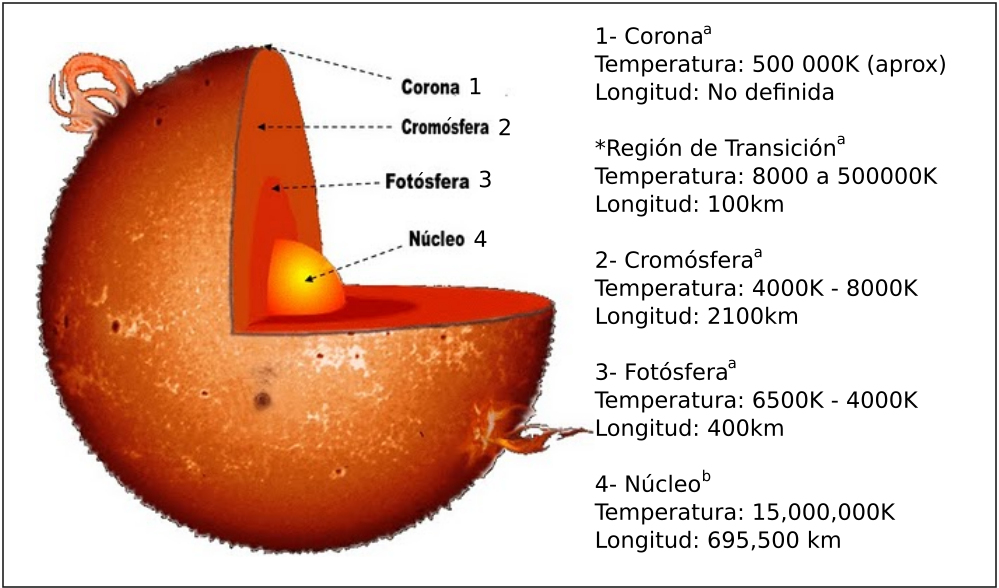
\includegraphics[scale=.5]{atmosfera}
\caption{ Representaci\'on gr\'afica de las capas del sol (no se encuentra a escala). \newline
*Existe debate sobre si la regi\'on de transici\'on es una regi\'on por s\'i misma o forma parte de la Crom\'osfera. Independientemente de esto, se localizar\'ia entre la Crom\'osfera y la Corona Solar. \newline
$^{a}$ https://www.nasa.gov/mission\_pages/iris/multimedia/layerzoo.html \newline
$^{b}$ https://solarscience.msfc.nasa.gov/interior.shtml}
\label{atmosfera_solar}
\end{figure}


%https://solar-energia.net/definiciones/sol.html

De entre estas la crom\'osfera es una de las partes m\'as desconocidas para la ciencia hasta el momento. Su mayor misterio es que conforme la densidad decrementa, la temperatura en lugar de decrementar tambi\'en, incrementa. Este fen\'omeno se presenta a\'un m\'as radicalmente en una regi\'on particular conocida como regi\'on de transici\'on (TR por su nombre en ingl\'es "Transition Region"). Particularmente, en dicha regi\'on resulta inexplicable el cambio radical que pasa de $10^4$K a $10^5$ K en una distancia de 1000km (Vease figuras \ref{d_cromosfera} y \ref{t_cromosfera}, donde se ilustran los cambios de densidad y temperatura).

\begin{figure}[h]
\centering
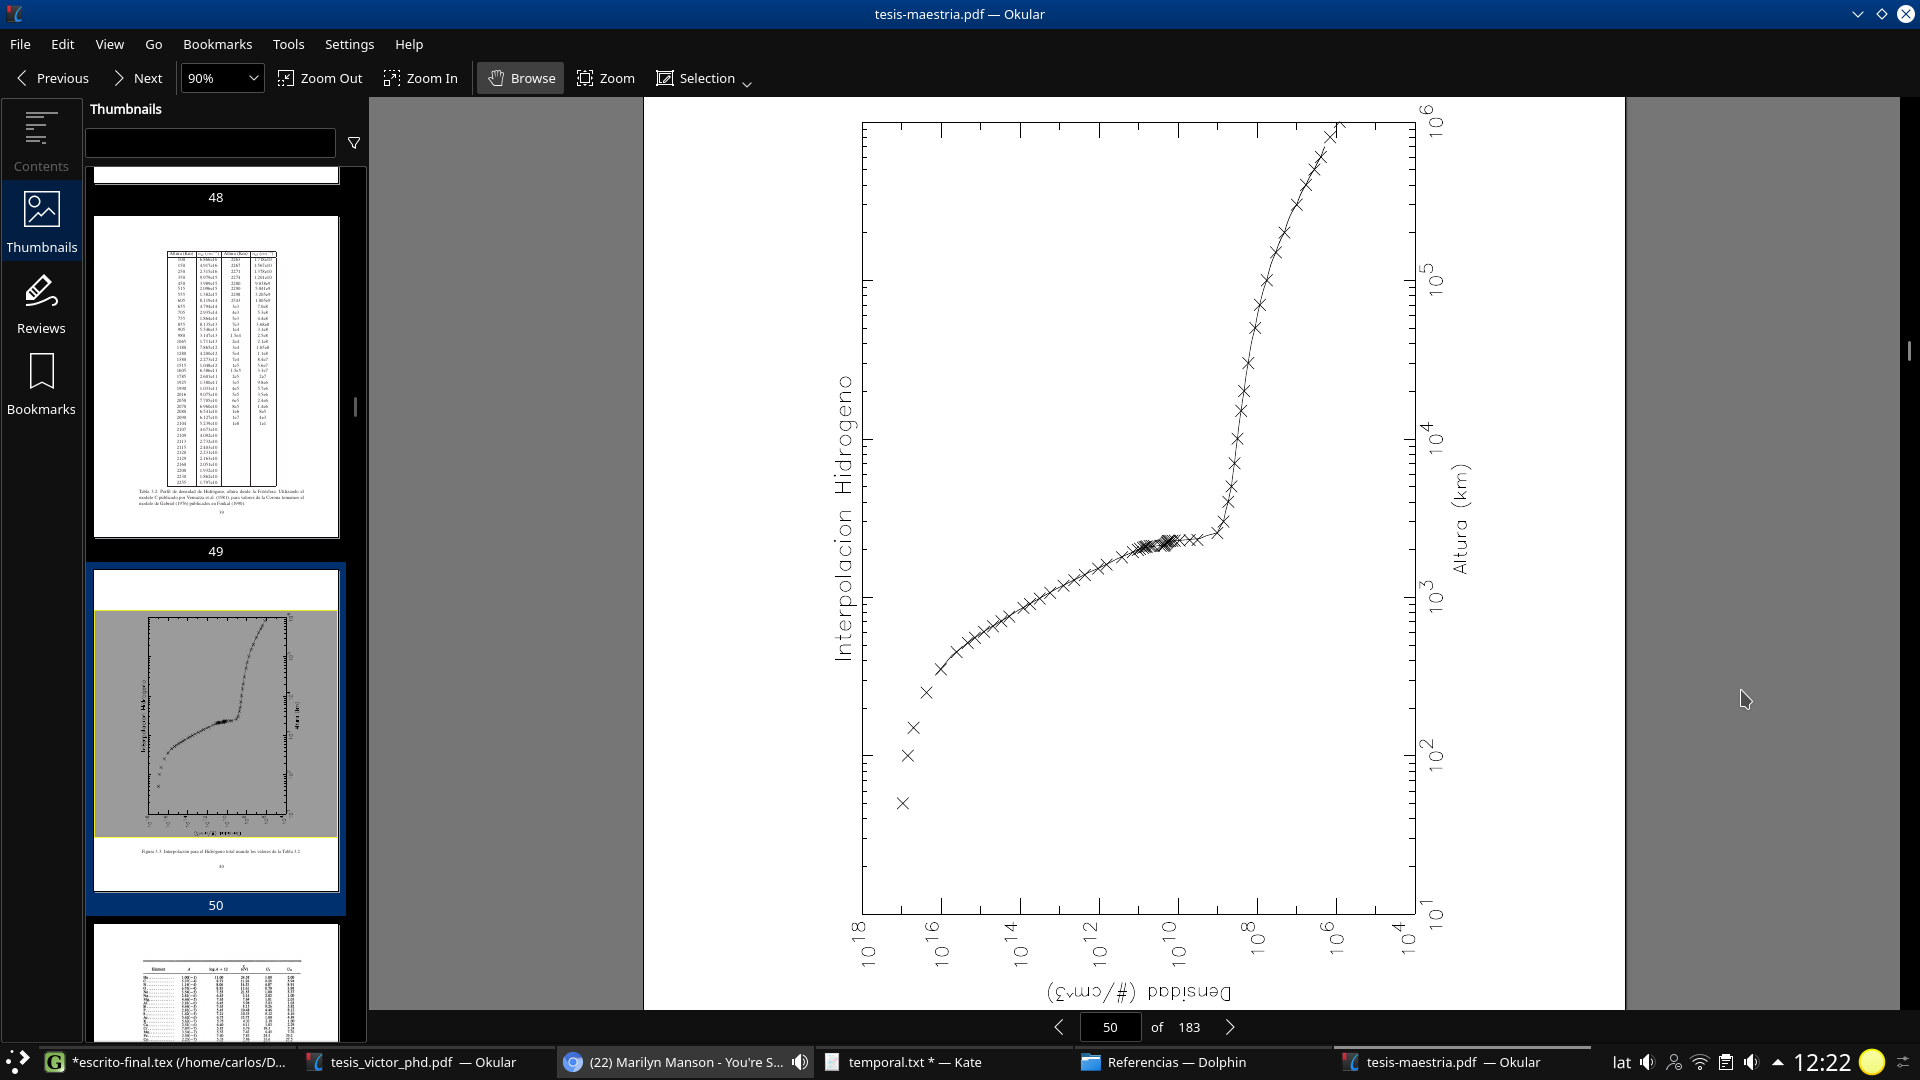
\includegraphics[scale=.8]{densidad}
\caption{ Perfil de densidad de Hidr\'ogeno, altura desde la Fot\'osfera utilizando el modelo C publicado por Vernazza (1981), para la Corona se toma el modelo de Gabriel (1976) (V de la Luz., 2011) }
\label{d_cromosfera}
\end{figure}

\begin{figure}[h]
\centering
\includegraphics[scale=.8]{Temperatura}
\caption{ Perfil de Temperatura, altura desde la Fot\'osfera utilizando el modelo C publicado por Vernazza (1981), para la Corona se toma el modelo de Gabriel (1976) (V de la Luz., 2011) }
\label{t_cromosfera}
\end{figure}


Como se mencion\'o anteriormente, existen distintas teor\'ias que tratan de explicar el cambio radical de temperatura en esta regi\'on. Una de ellas (PENDIENTE, revisar fuente) adjudica cierta causalidad a los campos magn\'eticos. Esta teor\'ia cobra cierta plausibilidad cuando se observa el sol mediante un espectr\'ografo o alg\'un filtro que aisle la emisi\'on H-alpha, que nos permite observar nuevas caracter\'isticas en las regiones del sol. Estas observaciones se han facilitado con el advenimiento de muevos instrumentos que observan en el rango UV, tales como IRIS (Interface Region Imaging Spectrograph). Con estas nuevas tecnolog\'ias y observaciones se ha descubiero que la estructura de la atm\'osfera (y muy particularmente, de la crom\'osfera) contienen una distribuci\'on ca\'otica. Actualmente los modelos de promedios, como VALC o C7, y que son los m\'as utilizados, no capturan la complejidad ca\'otica del escenario real.

Las nuevas tecnolog\'ias antes mencionadas nos han permitido entender mejor el comportamiento ca\'otico observado. Antes de su invenci\'on s\'olo pod\'iamos observar ciertas regiones del sol, como la crom\'osfera, durante un eclipse solar lo que limitaba nuestra investicaci\'on sobre la morfolog\'ia del sol. \'Unicamente se pod\'ia observar al sol durante los eclipses mencionados debido a que existe una capa muy brillante emitida por la fot\'osfera, que a causa de su intensidad de brillo enmascara las emisiones del resto de las regiones solares; sin embargo, cuando la luz de la fot\'osfera es filtrada el resto de las regiones m\'as d\'ebiles desaparecen tambi\'en por completo.

Hoy en d\'ia, con las nuevas tecnolog\'ias ya es posible la observaci\'on de detalles como la \emph{red cromosf\'erica}, donde se pueden observar peque\~nas estructuras de campos magneticos que pueden ayudar a explicar el comportamiento complejo concerniente.
La red cromosf\'erica se puede definir como una estructura en forma de micro arcos que forman una red oscura (network) que envuelve celdas brillantes (cells). Esta red es visible en espectroheliogramas tomados en la l\'inea H-alpha a una longitud de onda de cerca de 656 nan\'ometros y en otras regiones espectrales \cite{NASAweb}. Esta red rodea las celdas super granulares y consiste en un patr\'on de larga escala donde el movimiento del gas en la crom\'osfera es guiado por pliegues magn\'eticos (figura \ref{fig:chromosphericnet}). Las propiedades de la red cromosf\'erica justifican la exploraci\'on causal de campos magn\'eticos de esta tesis.

\begin{figure}[h]

\centering
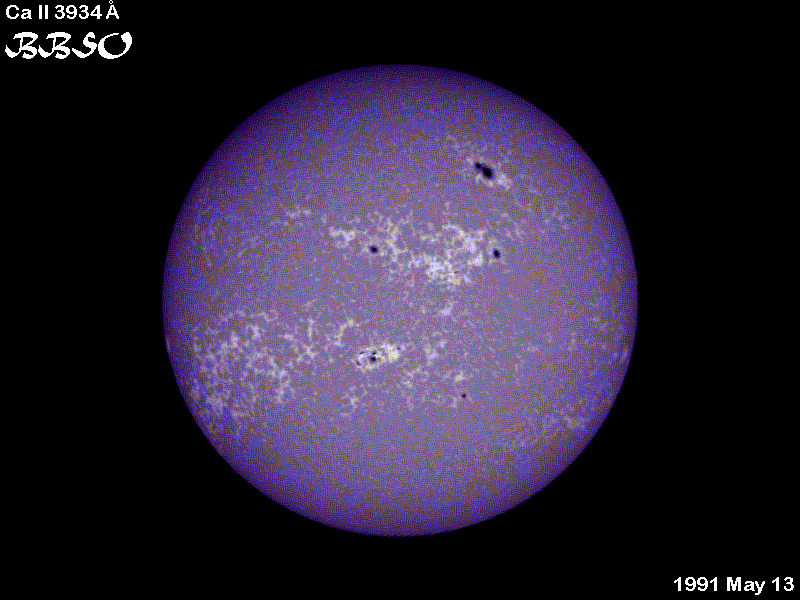
\includegraphics[scale=0.3]{CAII3934}
\caption{Fuente: The Chromospheric Network Mayo 2017, NASA p\'agina web oficial}
\label{fig:chromosphericnet}
\end{figure}

\begin{figure}[h]

\centering
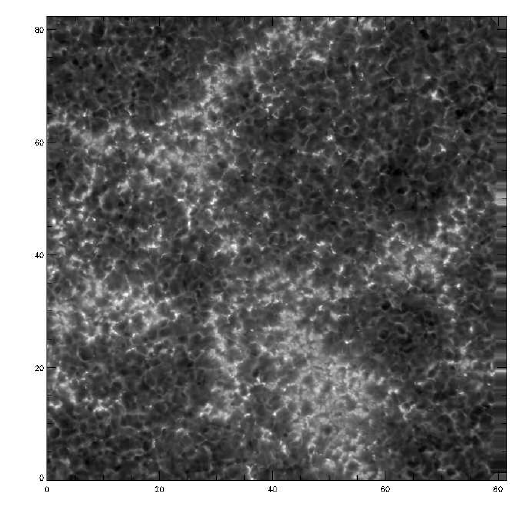
\includegraphics[scale=0.5]{chromospheric_network2}
\caption{ Red cromosf\'erica solar observada desde el Telescopio Solar Sueco (Swedish Solar Telescope) en la l\'inea H Ca II.
\newline Fuente: https://www.researchgate.net/figure/The-chromospheric-network-as-observed-with-the-Swedish-Solar-Telescope-in-the-Ca-II\_fig8\_259104617}
\label{chromospheric_network2}
\end{figure}

%En la figura \ref{fig:chromosphericnet} se observa una imagen tomada en la l\'inea de c\'alcio de la red cromosf\'erica, mientras que en la figura 

En a\~nadidura, las recientes observaciones del experimento VAULT (Very high Angular resolution ULtraviolet Telescope por sus siglas en ingl\'es) complementan la evidencia de una estructura ca\'otica cromosf\'erica y de la existencia de peque\~nos loops frios \cite{VAULT1}, los cu\'ales confirman la presencia de campos magn\'eticos.
VAULT es un proyecto de exploraci\'on espacial que data de 1999 y que busca estudiar la conexi\'on entre la corona y la crom\'osfera solar al observar la l\'inea espectral m\'as fuerte del sol, la Ly$\alpha$ a 1216A.
La resoluci\'on angular de subarcosegundos ($\approx$.3") permite ver directamente los peque\~nos loops f\'ios en la estructura de Sol Quieto. El parecido de los resultados entre los modelos y las observaciones indican que la explicaci\'on de las estructuras finas observadas en t\'erminos de loops frios es plausible.

Como se muestra en la figura x CORREGIR las im\'agenes de vault nos permiten mejorar la calidad de nuestras observaciones, permiti\'endonos tener un mejor entendimiento de la composici\'on de la atm\'osfera solar (n\'otese tambi\'en la calidad de la figura Y).

\begin{figure}[h]
\centering
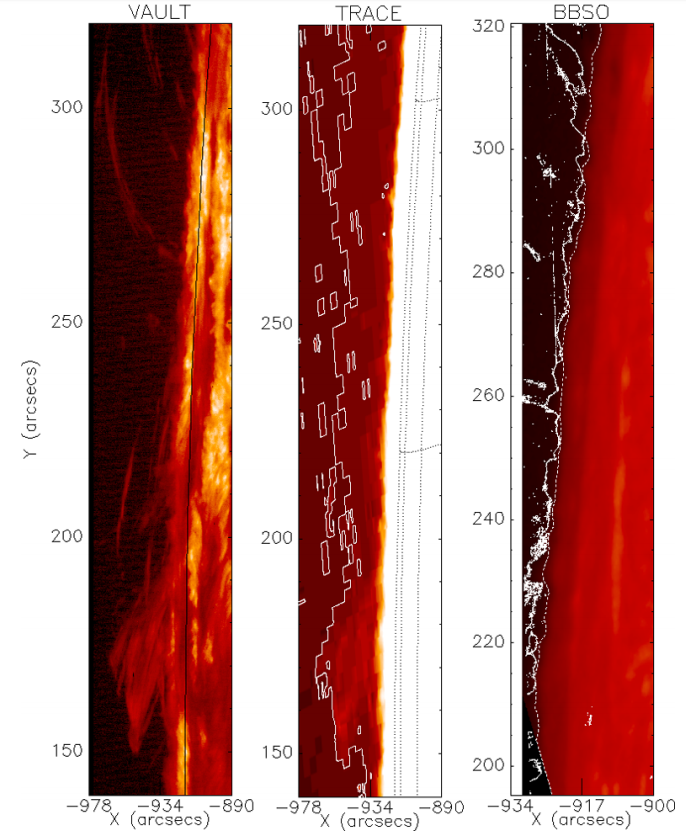
\includegraphics[scale=0.6]{vault_comparison}
\caption{"Fuente: Vourlidas, et al., 2009"}
\label{fig:vault_compare}
\end{figure}

\begin{figure}[h]
\centering
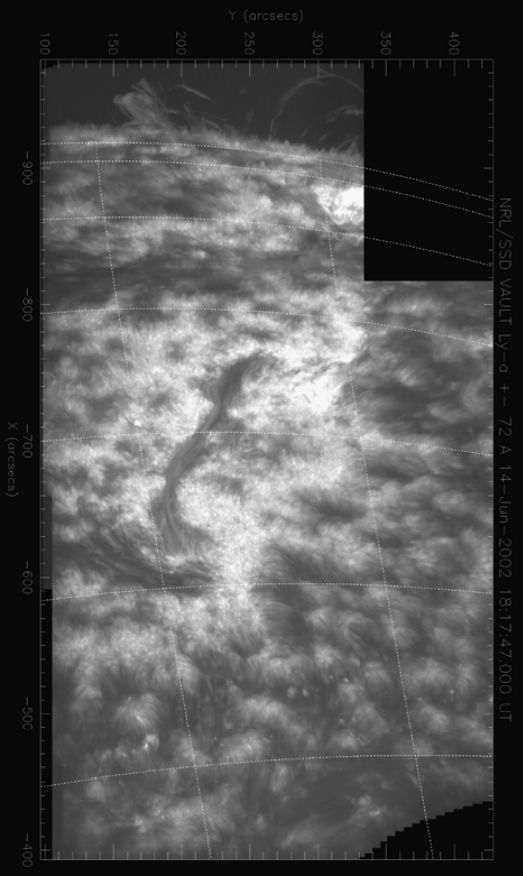
\includegraphics[scale=0.6]{vault_complete}
\caption{"Fuente: Vourlidas, et al., 2009}
\label{fig:vault_complete}
\end{figure}



\section{El c\'odigo \emph{PakalMPI}}
%Descripci\'on del c\'odigo, puntualmente hay qu\'e explicar primero para qu\'e sirve actualmente y a partir de ello, plantear las modificaciones.
Como se mencion\'o anteriormente, esta tesis busca extender el c\'odigo PakalMPI. Este programa fue constru\'ido por Victor de la Luz en el a\~no 2011\cite{PAKAL}. Dicho programa es un modelo num\'erico inovador que pretende resolver la ecuaci\'on de transferencia radiativa en una geometr\'ia tridimensional (3D), usando una aproximaci\'on para una atm\'osfera localmente plano paralelo; lo anterior utilizando un sistema inteligente. Con este programa se generan las capas estratificadas de la atm\'osfera en una estructura l\'ogica. La salida del c\'odigo puede ser en forma de mapas bi-dimensionales o un perfil de una dimensi\'on, que reproduce las observaciones con alta presici\'on, dando informaci\'on f\'isica detallada acerca del entorno donde la radiaci\'on fue generada y/o transmitida.

Pakal se encuentra dividido en cuatro distintos m\'odulos: El modelo num\'erico, la geometr\'ia, los m\'etodos num\'ericos y las funciones f\'isicas. Estos cuatro m\'odulos pueden ser modificados independientemente sin afectar el funcionamiento de los otros. En esta tesis se modifica el m\'odulo de las funciones f\'isicas donde se resuelve la ecuaci\'on de transferencia.

Como todo modelo, PakalMPI est\'a basado en una serie de supuestos que le brindan una serie de fortalezas, pero tambi\'en una serie de limitantes; las cuales se presentar\'an a continuaci\'on. Con relaci\'on a sus supuestos, PakalMPI presenta un modelo aplicado a una geometr\'ia solar radial 3D, asumiendo una atm\'osfera local plano-paralela, y una emisi\'on t\'ermica de radio libre-libre de gas hidr\'ogeno-helio en equilibrio termodin\'amico. Para sus c\'alculos Pakal asume un grosor de la Crom\'osfera de 2200km. Adem\'as tambi\'en utiliza perfiles radiativos precalculados de densidad y temperatura (basado en modelos hidrost\'aticos, hidrodin\'amicos o MHD) para calcular la emisi\'on de una fuente de estructuras 3D con alta resoluci\'on espacial. En todo momento PakalMPI asume un estado de Sol Quieto y la ausencia de campos magn\'eticos. El t\'ermino Sol Quieto hace referencia a regiones del Sol que se encuentran exentas de cualquier manifestaci\'on de actividad observable. Con los supuestos antes mencionados, el programa concerniente resuelve la ecuaci\'on de transferencia radiativa en un conjunto de l\'ineas dirigidas de la fuente al observador.

En relaci\'on con las limitaciones de PakalMPI, si bien este permite la entrada de observaciones, no est\'a basado en ellas, y por lo tanto los resultados que no representan por completo las caracter\'isticas f\'isicas. De igual forma, PakalMPI se encuentra limitado a la fot\'osfera y crom\'osfera, esto debido a que estas regiones presentan una baja actividad magn\'etica lo cu\'al permite despeciarla; contrario a lo que ocurrir\'ia en la corona solar. PakalMPI tambi\'en omite la emisi\'on \emph{gyrosynchrotron} al despreciar los campos magn\'eticos. Finalmente, el c\'odigo de PakalMPI no logra reproducir en un 100\% las funci\'ones de densidad y temperatura del plasma solar.
 
Finalmente como concerniente a sus fortalezas, PakalMPI ha demostrado poder mejorar el tiempo de integraci\'on hasta por un orden de magnitud comparado a c\'odigos de integraci\'on lineal. Por ejemplo, en una prueba que utilizaba 32 procesadores de una m\'aquina Cray del CNS en san Luis Potos\'i, se generaron espectros sint\'eticos de 32 frecuencias, con pasos de integraci\'on de 1km del centro del disco solar en aproximadamente 3 segundos. Adem\'as, PakalMPI puede correr en clusters, supercomputadoras y computadoras personales. Los resultados de PakalMPI han sido probados por su robustez. Particularmente, se realizaron satisfactoriamente pruebas de convergencia y estabilidad de la parte num\'erica y del sistema experto, las cu\'ales son presentadas en De la Luz et al. 2010. Por \'ultimo, PakalMPI permite modelar computacionalmente modelos emp\'iricos, te\'oricos y semi emp\'iricos. 

En esta tesis se propone una extensi\'on en el m\'odulo de funciones f\'isicas (denominado Jaguar). Particularmente se agrega el efecto de los campos magn\'eticos a la ecuaci\'on de transferencia al agregar la componente de la presi\'on magn\'etica. Lo anterior convierte al modelo hidrodin\'amico que se usa actualmente en un modelo magnetohidrodin\'amico. Con esta adici\'on ahora (1) se puede generar un escenario m\'as apegado a las observaciones f\'isicas de la atm\'osfera solar, y (2) se facilita la adaptaci\'on del c\'odigo ante la adici\'on de cualquier modelo de campo magn\'etico. Con relaci\'on a esto \'ultimo, ahora se puede solo cambiar una peque\~na fracci\'on del c\'odigo (la parte donde se encuentra el modelo de campo magn\'etico) sin necesidad de alterar el core de PakalMPI . 


\section{Sobre el Sol quieto y la emisi\'on submilim\'etrica solar}
%La resoluci\'on angular de subarcosegundos ($\approx$.3") permite ver directamente estructuras de la estructura de Sol Quieto. El parecido de los resultados entre los modelos y las observaciones indican que la explicaci\'on de las estructuras finas observadas en t\'erminos de loops frios es plausible.
Hist\'oricamente el concepto de Sol quieto se ha visto modificado, por lo que antes que todo se recomienda al lector tener precauci\'on en asumir una consistencia conceptual en textos de diferentes tiempos. Hoy en d\'ia, este t\'ermino se refiere a dos conceptos. Primeramente se puede referir a las regiones del Sol que abarcan todas las regiones de campo magn\'etico cerrado (excluyendo las regiones activas), claramente demarcando el territorio de Sol quieto de los hoyos coronales, que abarca regiones de campo magn\'etico abierto.
Segundamente, se refiere a un estado solar general que ocurre cada 11 a\~nos y se caracteriza por una actividad solar baja. Esta actividad solar baja b\'asicamente es equivalente a la primera definici\'on antes mencionada. En esta tesis cuando se utiliza el concepto de sol quieto, nos estamos refiriendo a la primer definici\'on, la cual describe el fen\'omeno solar de inter\'es. Se asume \'unicamente el estado de sol quieto debido a la complejidad del Sol activo. Sin embargo, el entendimiento del sol quieto tambi\'en nos ayudar\'ia a entender mejor el Sol Activo. Concretamente, la correcta caracterizaci\'on del Sol Quieto nos permitir\'ia entender el fondo de radiaci\'on del Sol Activo.

Una caracter\'istica relevante del Sol quieto para esta tesis es el de la intensidad de sus campos magn\'eticos. Particularmente los campos magn\'eticos en Sol quieto, medidos seg\'un las l\'ineas espectrales de Zeeman, contienen un campo de B== .1 - .5G, mientras que sus fuerzas absolutas de campo en elementos resueltos var\'ian entre B = 10-50G. Estos valores se utilizan en el modelo computacional propuesto en este texto.

Si bien se conocen los rangos de la magnitudes de los campos magn\'eticos del Sol quieto, existe una dificultad en medir las magnitudes concretas de estos debido a corrientes desconocidas y condiciones no libres de fuerza. Lo anterior ocasiona que se tengan que calcular extrapolaciones a lo largo de la crom\'osfera y la regi\'on de transici\'on para obtener valores aproximados. Sin embargo, estas mediciones extrapoladas contienen ruidos, lo que las hace imprecisas. Lo anterior justifica que el modelo presentado en esta tesis tome valores de campos magn\'eticos no concretos.

Otra caracter\'istica importante del Sol quieto para esta tesis es la emisi\'on milim\'etrica del plasma. Se ha comprobado que la observaci\'on de la emisi\'on milim\'etrica del plasma en Sol Quieto es equivalente a observar la totalidad de las emisiones de la Crom\'osfera Solar cuando est\'a en el estado solar de Sol Quieto 2000ESASP.463..363L. Con la emisi\'on milim\'etrica se puede aproximar el grado de ionizaci\'on de toda la atm\'osfera solar; y con esta \'ultima se pueden inferir aproximaciones de la temperatura, la densidad y la presi\'on que hay en ella. Estas \'ultimas aproximaciones se realizan seg\'un diferentes modelos; los cuales se pueden conceptualizar como emp\'iricos, semi-emp\'iricos y observacionales. 

Independientemente del tipo de modelo, por definici\'on, todos tienen limitaciones en sus c\'alculos de temperatura, densidad y presi\'on. En el modelo propuesto, se busca robustecer el modelo PakalMPI de V\'ictor de la Luz mediante la anexi\'on de el efecto te\'orico de los campos magn\'eticos. Esta anexi\'on se puede justificar, por diferentes teor\'ias y observaciones. Por ejemplo, un estudio reciente por Meunier (2018) propone que las peque\~nas regiones de campo magn\'etico contribuyen significamente a la emisi\'on cromosf\'erica y por consiguiente a la emisi\'on milim\'etrica. Lo anterior, como se explic\'o previamente, afectar\'ia a los c\'alculos de la temperatura, la densidad y la presi\'on de la crom\'osfera; haci\'endolos te\'oricamente m\'as precisos.

\chapter{Extensi\'on al modelo Pakal \-- A\~nadiendo presi\'on magn\'etica}

La extensi\'on propuesta en esta tesis al modelo computacional PakalIMPI le a\~nade a este \'ultimo el efecto de la presi\'on magn\'etica a la ecuaci\'on de estado. Con lo anterior, el modelo de PakalIMPI, que en principio era un modelo computacional que simulaba un modelo hidrost\'atico para el comportamiento del plasma, se robustece al convertirse en un modelo de Magnetohidrost\'atica. Hablando en t\'erminos f\'isicos, se podr\'ia decir que el modelo original resolv\'ia la siguiente ecuaci\'on de estado:

**** PONER FORMULITA de vic de hidrost\'atica***

A esta f\'ormula, se le a\~nade el efecto de la presi\'on magn\'etica, resultando en la siguiente ecuaci\'on ****CITAR CORREGIR**.

****PONER FORMULITA MHD CORREGIR***

Cabe aclarar que la f\'ormula que utiliza el c\'odigo de la extensi\'on a PakalIMPI considera la siguiente ecuaci\'on de presi\'on magn\'etica para realizar los c\'alculos:

$PB = \frac{B^2}{8\Pi}$

A continuaci\'on se precisar\'a el c\'odigo de la extensi\'on computacional al programa PakalIMPI realizado en esta tesis. Se contextualizar\'a dicho c\'odigo con secciones del c\'odigo original. Las extensiones al c\'odigo se diferenciar\'an al c\'odigo original al estar con un estilo de letra en \textbf{negrita}, mientras que los nombres de los archivos se encuentran \underline{subrrayados}. Adem\'as, se comentar\'a la funci\'on realizada por el c\'odigo agregado. 

Para hacer posible la adici\'on del efecto de la presi\'on magn\'etica sobre la ecuaci\'on de estado dentro del c\'odigo Pakal, se modificaron los siguientes archivos:\newline \newline \newline \newline

\underline{hmodel.h}
En esta libreria se definen la estructura de la atmosfera, a la cual se le agregaron las componentes x, y, z del campo magnetico, asi como la variable xi para la modulacion del mismo
\begin{lstlisting}[style=CStyle]
typedef struct{
	int id;
	double z;
	double T;
	double P;
	double H;
	double V;
	double vt;
	double ne;
	double ne_lte;
	double bhm;
	double fz;
	/*-------------------------------------------------------------*/
	//Se agregan las componentes del campo y xi
	double Bx;
	double By;
	double Bz;
	double xi;
	/*-------------------------------------------------------------*/	
}Atmosphere;

\end{lstlisting}

\underline{main.c}
Esta es la parte donde el m\'odulo Jaguar se encarga de llamar a las respectivas funciones que llevan a cabo los c\'alculos de cada uno de los pasos de integraci\'on. En este c\'odigo se agreg\'o la lectura de los valores de campo.\newline
Los parametros amplitud e intensidad son los respectivos valores del campo magnetico.\newline
El par\'ameto alpha se define en el capitulo 4.\newline
El par\'ametro B\_x0 representa la altura a la que nace el campo magn\'etico, tomando como referencia la base de la fot\'osfera.
\begin{lstlisting}[style=CStyle]

int main(int argc, char **argv){
	int i,j;
	Model model;
	char env[500];
	char comando[500];
	double hydro_step;
	double pz1;
	double Y;
	double fz1;
	double dx;
	int chromospheric_network;
	int cell;
	int hydro;
	/*----------------------------------------------------------*/
	//Los parametros amplitud e intensidad son los respectivos valores del campo magnetico
	//El parametro alpha representa el angulo entre el nacimiento del campo magnetico y el punto que se desea calcular, tomando como referencia de centro el centro solar
	//B_x0 representa la altura de nacimiento del campo, tomando como referencia la base de la fotosfera
	//magnetic es la variable que nos dice si se llamo la bandera del campo magnetico
	double amplitude, intensity, alpha;
	int magnetic = 0;
	int B_x0;
	/*----------------------------------------------------------*/

	printf("Loading Atomic Model:\n");
	model = newModel(argv[1]);
	chromospheric_network=0;
	hydro = 0;

	for (i=1; i<argc; i++) {
		sprintf(comando,"%s",argv[i]);
		if (strcmp(comando,"-hydro") == 0) {
			hydro= 1;
		}

		if (strcmp(comando,"-cn") == 0) {
			sprintf(comando,"%s",argv[++i]);
			if (sscanf(comando,"%i\n",&cell) > 0) {
				chromospheric_network=1;
				printf("Error: Network or cell is required.\n");
				return 0;
			}
		}
		/*-----------------------------------------------------------*/	
		//Aqui se lee la bandera del campo magnetico representada por -B y se transfieren al codigo los parametros de entrada
		if (strcmp(comando, "-B") == 0) {
			sprintf(comando, "%s",argv[++i]);
			if(sscanf(comando,"%lf\n",&amplitude) > 0) {
				sprintf(comando, "%s", argv[++i]);
				if(sscanf(comando,"%lf\n",&intensity) > 0) {
					sprintf(comando, "%s", argv[++i]);
					if(sscanf(comando,"%lf\n",&alpha) > 0) {
						sprintf(comando, "%s", argv[++i]);
						magnetic = 1;
					}
				}
			}
		}
		/*----------------------------------------------------------*/	
	}

	B_x0 = 1;
	loadInitValues(&model, 0);
	if(magnetic == 1) {
		init_B(amplitude, intensity, alpha, &model, B_x0);
	}
	printf("Layer 0\n");
	NLTE(&model,1e-14,0,0.0,0.0,0.0,chromospheric_network,cell,0);
	writeModel(model,"dummy/");

	for (i=1; i<= model.n; i++) {
		pz1 = model.atm.P;
		fz1 = model.atm.fz;
		dx = model.atm.z;
		loadInitValues(&model, i);
		/*----------------------------------------------------------*/	
		//En caso de que la bandera haya sido activada, se calcula el campo magnetico y modidica directamente los valores de las capas de la atmosfera por medio del parametro &model.
		if(magnetic == 1) {
			calculate_B(amplitude, intensity, alpha, &model, B_x0);
		}
		/*----------------------------------------------------------*/	
		if (!(hydro)) {
			printf("Layer %i (ion)\n",i);
			/*---------------------------------------------------------*/	
			//Dado que la opcion hydro no fue activada, se asume que no se busca tampoco el campo magnetico (esto se representa por el 0 del final)
			/*---------------------------------------------------------*/	
			NLTE(&model,1e-14,0,0.0,0.0,0.0,chromospheric_network,cell,0);
		}else{
			printf("Layer %i (hydro)\n",i);
			dx = model.atm.z - dx;
			/*---------------------------------------------------------*/	
			//Si la opcion hydro fue activada, se le pasa al modelo NLTE el parametro "magnetic"
			/*---------------------------------------------------------*/	
			NLTE(&model,1e-14,1,pz1,fz1,dx,chromospheric_network,cell,magnetic);
		}
		writeModel(model,"dummy/");
	}
	return 0;
}
\end{lstlisting}

\underline{nlte.c}
Esta seccion resuelve la ecuaci\'on de estado con un modelo NLTE (non local thermodynamic equilibrium), y es donde se agrega como tal la influencia de la presi\'n magn\'etica
\begin{lstlisting}[style=CStyle]

#include <string.h>

double totalParticles =0.0;
double magnetic_true = 0;

/*---------------------------------------------------------*/
//Es aqui donde se resuelve la funcion de estado, por lo que es donde se realiza la principal contribucion de esta tesis.

double f_hydro(double Y, double R, double Z, double T, double vt, double bx, double by, double bz, double xi){
	//g * m_H 6.674e-8 cm^3g-1s-2 * 1.673534e-24 g
	double R1,KT,R2,R3,R4,R5,R6,B, magnetic_field;


	//Se agrega un archivo que contiene los valores del campo magnetico y de la presion a cada altura, para poder observarlos y graficarlos de ser necesario. Los valores se encuentran contenidos en el archivo magnetic_and_pressure.dat
	char tmp_name[300];
	FILE *tmp_file;
	strcpy(tmp_name,"magnetic_and_pressure.dat");
	//De momento solamente se toma en cuenta la componente z del campo magnetico, por lo que esta se asigna al valor del campo
	magnetic_field = bz;

	if(magnetic_true != magnetic_field)
	{
		tmp_file = fopen(tmp_name,"a");
		magnetic_true = magnetic_field;
		printf("magnetic_field=%le\n",magnetic_field);
		fprintf(tmp_file, "%le   %le\n", 0.0, xi*magnetic_field/(8*M_PI));
		fclose(tmp_file);
	}
	first_time = 1;
	//Esta es la ecuacion resultante con la componente del campo magnetico (xi*magnetic_field/(8*M_PI))
	B = 1.0+R+Y+Z+( (0.5*pow(vt,2.0)*(1.0+4.0*Y)*mH)/(kboltz*T)) + xi*magnetic_field/(8*M_PI);

//B = 1.0+R+Y+Z+( (0.5*pow(vt,2.0)*(1.0+4.0*Y)*mH)/(kboltz*T));
//Esta era la ecuacion antes de ser modificada

	return exp(log(GMH) - log(kboltz*T) + log(1.0+4.0*Y) - log (B));

}
/*---------------------------------------------------------*/

\end{lstlisting}

\underline{nlte.h}
En el encabezado de la libreria de NLTE (non local thermodynamic equilibrium) se modifica para aceptar el campo magnetico
\begin{lstlisting}[style=CStyle]
//Se agregan las componentes x, y, z y xi para ser introducidas en la ecuacion de estado
double f_hydro(double Y, double R, double Z, double T, double vt, double bx, double by, double bz, double xi);
void NLTE(Model *model, double error, int hydro, double pz1, double fz1,double dx, int chromospheric_network,int cell, int magnetic);
\end{lstlisting}

\underline{pakal.c}
Pakal, al ser la parte del c\'odigo que "interact\'ua" con el usuario, es la parte que procesa la informaci\'on de la terminal y la env\'ia al resto del c\'odigo, tomando como entrada de la terminal los valores amplitud, intensidad y alpha, que son respectivamente los valores que se introduciran al campo magn\'etico.
Amplitud: La amplitud del campo
Intensidad: La intensidad del campo
Alpha: \'Angulo entre el nacimiento del campo y la l\'inea de visi\'on a la que se desea calcular
\begin{lstlisting}[style=CStyle]
/*---------------------------------------------------------*/
//campo magnetico
double B_amplitude = 0, B_intensity = 0, B_alpha = 0;
int magnetic = 0;
//componente de campo magnetico
if (strcmp(comando,"-B") == 0) {
	sprintf(comando,"%s",argv[++i]);
	if (sscanf(comando,"%lf\n",&B_amplitude) > 0) {
		sprintf(comando,"%s",argv[++i]);
		if (sscanf(comando,"%lf\n",&B_intensity) > 0) {
			sprintf(comando,"%s",argv[++i]);
			if(sscanf(comando,"%lf\n",&B_alpha) > 0) {
				magnetic=1;
			}
			else{
				imprimeInstrucciones();
				return 0;
			}
		}
		else{
			imprimeInstrucciones();
			return 0;
		}
	}
	else{
		imprimeInstrucciones();
		return 0;
	}
}
/*----------------------------------------------------------*/

if (!(compute_ion_profile)) {
	if (hydro) {

		sprintf(comando,"rm data/atmosphere/chromosphere/average/*.dat");
		system(comando);
		printf("Computing hydrostatic atmosphere.\n");

		if(magnetic) {
			sprintf(comando,"jaguar/jaguar %s -hydro -B %le %le %le",atm_model, B_amplitude, B_intensity, B_alpha);
		}
		else{
			sprintf(comando,"jaguar/jaguar %s -hydro",atm_model);
		}

		system(comando);

		printf("Ready\n");
		return 0;
	}else{
		printf("Using previous ion profiles.\n");
	}
}else{
	if (chromosnet) {
		printf("Computing ion profiles CN activated.\n");
		sprintf(comando,"rm data/atmosphere/chromosphere/chromosnet/cell/*.dat");
		system(comando);
		sprintf(modelCell,"%s-CELL",atm_model);
		printf("Computing %s \n", modelCell);
		sprintf(comando,"jaguar/jaguar %s -cn 1",modelCell);   
		printf("%s\n",comando);
		system(comando);
		printf("Ready\n");
		printf("Computing ion profiles.\n");
		sprintf(comando,"rm data/atmosphere/chromosphere/chromosnet/net/*.dat");
		system(comando);
		sprintf(modelNet,"%s-NET",atm_model);
		printf("Computing %s \n", modelNet);
		sprintf(comando,"jaguar/jaguar %s -cn 0",modelNet);
		printf("%s\n",comando);
		system(comando);
		printf("Ready\n");
		return 0;
	}else{
		printf("Computing ion profiles.\n");
		sprintf(comando,"rm data/atmosphere/chromosphere/average/*.dat");
		system(comando);
		sprintf(comando,"jaguar/jaguar %s",atm_model);
		printf("%s\n",comando);
		system(comando);
		printf("Ready\n");
		return 0;
	}
}
\end{lstlisting}
  
\chapter{Pruebas a la extensi\'on de PakalIMPI y sus Resultados}

Para probar la extensi\'on realizada al modelo computacional PakalIMIPI en esta tesis en esta tesis, se llevaron a cabo la simulaci\'ones del comportamiento de los campos magn\'eticos seg\'un dos modelos distintos. Uno en forma de arcos magn\'eticos \cite{loops} y otro en forma de un flujo emergente \cite{flujoemergente}. A continuaci\'on se precisar\'an las caracter\'isticas f\'isicas que se presuponen en cada modelo; as\'i como los resultados obtenidos para cada caso tras la simulaci\'on computacional.

\section{Caracter\'isticas F\'isicas de los modelos de prueba \- Arcos Magn\'eticos y Flujo Emergente}

Cabe se\~nalar que se eligieron estos dos modelos de campos magn\'eticos por diversas razones. Primeramente, se utilizaron los supuestos de los Arcos Magn\'eticos debido a que en algunas observaciones del experimento VAULT \cite{VAULT}, se observaron peque\~nas y relativamente fr\'ias estructuras cromosf\'ericas (LRI CORREGIR(aprox) 0.2); las cuales, hasta el momento, han sido las m\'as peque\~nas y con menor temperatura encontradas (v\'ease Anexo es del paper de VAULT2 CORREGIR). El origen de estas estructuras a\'un son un misterio, pero se ha teorizado que podr\'ian ser loops fr\'ios\cite{VAULT2}. El modelo de arcos magn\'eticos intenta representar estos loops fr\'ios. Por su parte, se realiza la simulaci\'on computacional bajo el modelo de campos magn\'eticos seg\'un la teor\'ia de Flujos Emergentes (Judge, 2008 CORREGIR) porque algunas observaciones (citar SUMER CORREGIR) parecen proveer de evidencia de que los campos magn\'eticos se pueden comportar seg\'un lo descrito por la teor\'ia concerniente. 

\subsection{Arcos Magn\'eticos}

Para este modelo el programa utiliza 3 par\'ametros de entrada: (1) la altura con respecto a la base de la fot\'osfera donde nace el campo magn\'etico, (2) el momento magn\'etico, y (3) el par\'ametro $\alpha$. Por medio de trigonometr\'ia, se encuentra adem\'as la relaci\'on entre los par\'ametros antes mencionados; obteni\'endose y los valores r y $\theta$ (v\'eanse Figura \ref{arco_geometria} y Figura \ref{arco_magnetico} ). A continuaci\'on se detallan las propiedades f\'isicas pertinentes para este modelo.

Los siguientes 3 valores son los que toma como entrada el programa Pakal, por lo que pueden ser modificados por el usuario.

\textbf{Altura de nacimiento del campo (l)}. Significa la distancia desde el centro del sol hasta el punto donde nace el arco magn\'etico (el conductor enterrado, de acuerdo al modelo de arcos magn\'eticos. Ver Figura \ref{arco_geometria}). El valor utilizado es un supuesto arbitrario bajo par\'ametros deductivos seg\'un caracter\'isticas de la fot\'osfera. Particularmente, debido a que el modelo de arcos magn\'eticos asume que la fuente de este campo es un conductor, se deduce que \'este tendr\'ia que estar enterrado debajo de la superficie de la fot\'osfera, ya que si estuviera por encima podr\'ia ser observado con diferentes tecnolog\'ias (como VAULT). Por lo tanto, se consider\'o que el conductor existe entre 150 km debajo.

\textbf{Momento magn\'etico (m).} Es la fuerza y orientaci\'on magn\'etica de un im\'an o cualquier objeto que produce un campo magn\'etico. Para el momento magn\'etico se utiliz\'o un valor de $2.5964x10^{12}$Mx (solar\_chromosphere). Este valor ha sido probado emp\'iricamente, y demostr\'o ser observacionalmente aproximado a los valores te\'oricos, sin embargo es un par\'ametro que el c\'odigo toma como entrada y puede ser variado.

\textbf{alpha ($\alpha$).} Se refiere al \'angulo que se forma entre el nacimiento del arco magn\'etico y el punto que se desea calcular, tomando como referencia base el centro solar (Ver Figura \ref{arco_geometria}). Este valor fue calculado de tal forma que Theta arrojara un n\'umero muy cercano a 92\degree.

Los siguientes valores son valores que se calculan por el mismo programa Pakal y son invisibles para el usuario, sin embargo son utilizados para los c\'alculos del campo magn\'etico.


\textbf{\(R\odot\)}  representa al radio solar y se toma un redondeo a $6.96x10^8m$.

\textbf{h.} Representa la distancia desde el punto cuyo campo magn\'etico se busca calcular hasta el centro solar, menos el radio solar (Ver Figura \ref{arco_geometria}). Este valor se toma seg\'un lo arrojado por el c\'odigo PakalMPI sin la extensi\'on propuesta en esta tesis.

\textbf{Theta ($\theta$). }Es el \'angulo que se forma entre la base del nacimiento del arco y el punto que se desea calcular. Las pruebas para el \'angulo Theta utilizado fue seleccionado arbitrariamente en 92\degree para poder reflejar el mayor cambio determinable en el campo magn\'etico (seg\'un el modelo de Arcos Magn\'eticos) dada la resoluci\'on computacional utilizada (8 bytes de un double del lenguaje C). Te\'oricamente el mayor cambio en un campo magn\'etico ocurre en el \'angulo de 90\degree, pero la intensidad del campo magn\'etico resulta indeterminado con este valor de Theta seg\'un la ecuaci\'on de la intensidad del campo (CORREGIR refi\'erase a Anexo 3); adem\'as debido al redondeo de valores y a las grandes magnitudes utilizadas, los valores arrojados entre 89 y 91 generaron tambi\'en valores indeterminados. Sin embargo el software est\'a preparado para recibir cualquier valor.\newline
La relaci\'on entre este \'angulo y el \'angulo $\alpha$ que es el que utiliza Pakal fue determinado por la ley de senos con las siguientes ecuaciones:
\begin{gather*} \label{theta_equation}
\frac{r}{sen(\alpha)} = \frac{d}{sen(\omega)} \\
\omega = sen^{-1}(\frac{(d)(sen(\alpha))}{r}) \\
\alpha + 90 + \theta + \omega = 180 \\
\theta = 90 - \alpha - \omega
\end{gather*}

\textbf{r. }Representa la distancia medida en l\'inea recta desde el nacimiento del campo magn\'etico hasta el punto cuyo valor de campo se desea calcular. Este valor se calcula de acuerdo de valor h por medio de la ley de cosenos con la f\'ormula
 
\begin{equation*} \label{r_equation}
r = \sqrt{ (h+R)^2 + (d)^2 - 2(h+R)(d)cos(\alpha)  }
\end{equation*}

\begin{figure}[h]
\centering
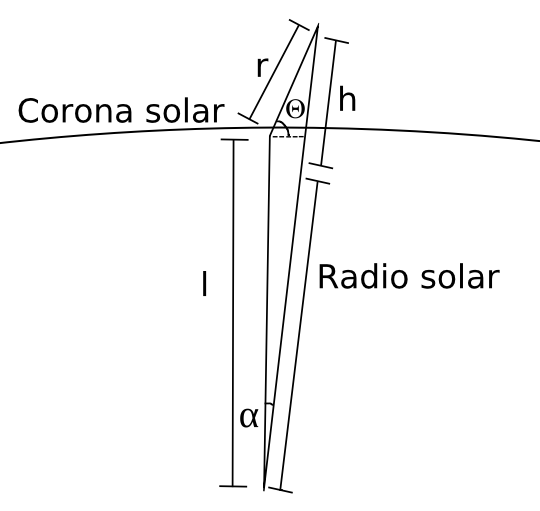
\includegraphics[scale=.8]{arco_magnetico_geometria}
\caption{ Representa la geometr\'ia que se utiliza para adaptar los par\'ametros del arco magn\'etico. }
\label{arco_geometria}
\end{figure}

\begin{figure}[h]
\centering
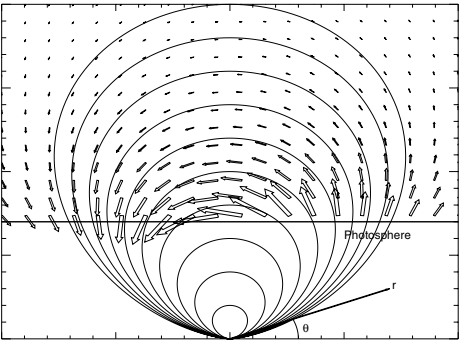
\includegraphics[scale=.8]{magnetic_loop}
\caption{ Imagen tomada del Aswanden. Representa el modelo de arco magn\'etico, donde la longitud de las flechas indican la intensidad del campo, y la direcci\'on en la que apuntan corresponde a la del campo. }
\label{arco_magnetico}
\end{figure}
\clearpage

\subsection{Flujo Emergente}

\textbf{Escala de altura (h). }Es un valor emp\'irico que permite determinar qu\'e tanto se difumina el campo magn\'etico con respecto a la altura. Su valor fue seleccionado de tal forma que los rangos de sus valores caigan dentro de los emp\'iricos que han sido observados. Concretamente, el rango de observaciones emp\'iricas va de 500 a 1000G \cite{VAULT} y para realizar la prueba se tom\'o aleatoriamente el de valor de 200.

\textbf{Flujo magn\'etico (phi). }Representa el campo magn\'etico total que pasa por un \'area determinada. Para realizar las pruebas a la extensi\'on computacional propuesta, se tom\'o como valor del flujo magn\'etico $\phi=2.8x10^{18}$Mx. Si bien existe debate sobre las aproximaciones m\'as precisas con respecto a este valor \cite{magneticflux}; se consider\'o \'este debido a que los resultados del radio inicial del tubo de flujo del modelo de Flujo Emergente fueron coherentes con la teor\'ia (366km \cite{magneticflux} y \cite{VAULT}) al utilizarlo.

\textbf{Intensidad de campo inicial en su base (B0). }Se refiere al valor que toma el campo magn\'etico en la base de su nacimiento, o desde el punto donde se desea comenzar a medir. Los c\'alculos fueron generados considerando distintos valores de campo magn\'etico (0, 500, 1000 y 1500 Gauss), dado que en la literatura se ha dado este valor entre 1000 y 1500 Gauss. La fuerza de la red cromosf\'erica es 1 kG a z=0 con una altura de 500km de acuerdo a Judge (2006 CORREGIR).

\clearpage
\section{Resultados}

En esta secci\'on se presentar\'an los resultados obtenidos de las simulaciones seg\'un los modelos de arcos magn\'eticos y flujo emergente.

\subsection{Micro arco magnetico}
El modelo de arcos magn\'eticos es uno de los modelos m\'as simples y m\'as irreales para simular el comportamineto solar. Sin embargo, a su vez, es un modelo que facilita la comprensi\'on y vizualicaci\'on de la morfolog\'ia del campo magn\'etico de una manera pedag\'ogica.

Los primeros resultados que se presentan, son aquellos concernientes a las pruebas de la codificaci\'on del modelo de arcos magn\'eticos para obtener lo perfiles de los propios arcos magn\'eticos. Particularmente, se realizaron pruebas en los campos magn\'eticos iniciales de 0, 25, 183 y 570G. Con estos valores se obtuvo un perfil del campo magn\'etico a lo largo de la altura; cuyos resultados se pueden apreciar en la Figura \ref{am_Campo_Magnetico}. Como se puede observar, los valores de los campos magn\'eticos arriba de los 1,000 km terminan siendo relativamente peque\~nos, independientemente del valor de entrada. Lo anterior va acorde a la teor\'ia del campo magn\'etico de la crom\'osfera.

Una vez obtenidos los perfiles de los arcos magn\'eticos, ya se puede ajustar la presi\'on de la crom\'osfera a diferentes alturas. Los resultados obtenidos a trav\'es de la extensi\'on al c\'odigo PakalMPI se representan en la Figura \ref{am_Presion}. En ella se puede ver que conforme m\'as grande es el campo magn\'etico, la presi\'on decrementa menos, manteni\'endose a un valor m\'as alto. 

Despu\'es de obtener los resultado de la presi\'on de la crom\'osfera, se pueden calcular los valores de la densidad del hidr\'ogeno presente en la crom\'osfera. Estos resultados se pueden apreciar en el gr\'afico \ref{am_perfil_de_densidades}. Como se puede observar el comporamiento general es que a mayor campo magn\'etico menor es el gradiente de la densidad. En adici\'on a estos resultados, se muestran tambi\'en dos comparativos entre los resultados de las densidades para diferentes campos magn\'eticos. Estos \'ultimos resultantes se grafican en la Figura \ref{am_diferencias_absolutas} y en la Figura \ref{am_diferencias_relativas}.

\newpage
\begin{figure}[h]
\centering
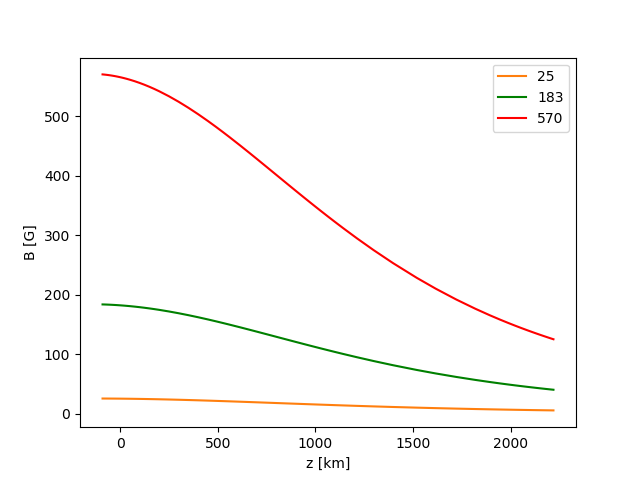
\includegraphics[scale=1]{am_Campo_Magnetico}
\caption{ En esta gr\'afica se describe el comportamiento de la intensidad del campo magn\'etico. }
\label{am_Campo_Magnetico}
\end{figure}


\begin{figure}[h]
\centering
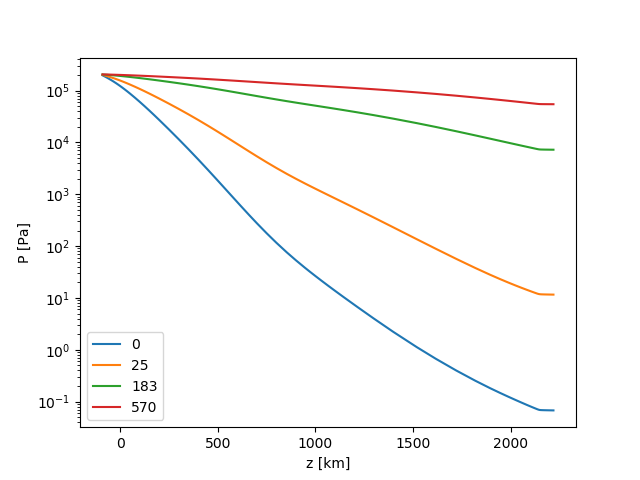
\includegraphics[scale=1]{am_Presion}
\caption{ Aqu\'i se presentan cada una de las salidas de las simulaciones con los distintos valores de campo magn\'etico seg\'un los resultados anteriores.}
\label{am_Presion}
\end{figure}

\begin{figure}[h]
\centering
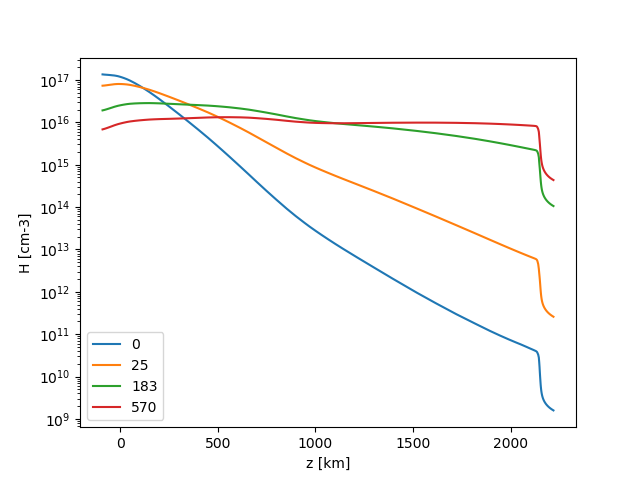
\includegraphics[scale=1]{am_perfil_de_densidades}
\caption{ En esta figura se grafican el perfil de densidades de hidr\'ogeno.}
\label{am_perfil_de_densidades}
\end{figure}

\begin{figure}[h]
\centering
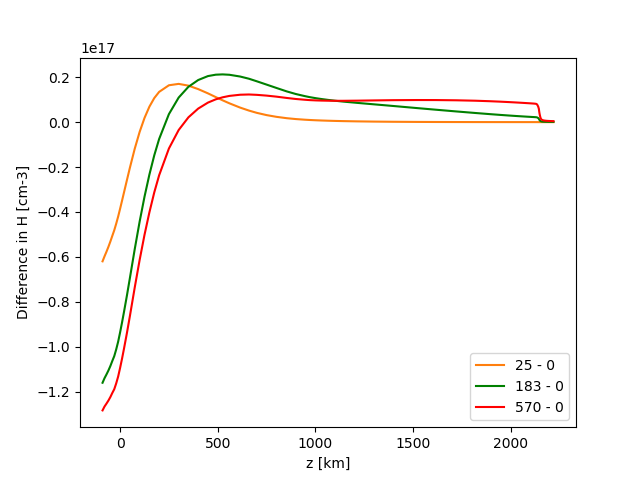
\includegraphics[scale=1]{am_diferencias_absolutas}
\caption{ Aqu\'i se muestra una comparaci\'on entre las diferentes salidas de las densidades del programa.}
\label{am_diferencias_absolutas}
\end{figure}

\begin{figure}[h]
\centering
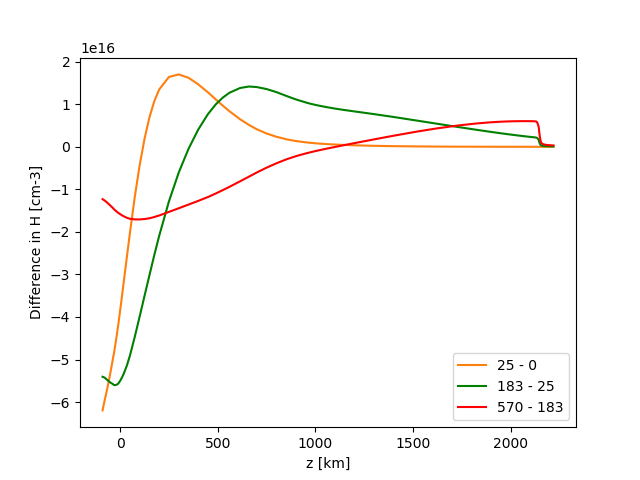
\includegraphics[scale=1]{am_diferencias_relativas}
\caption{ Aqu\'i se muestra un diferencial de cada uno de las salidas de las simulaciones contra las salidas de la simulaci\'on con un valor m\'as bajo.}
\label{am_diferencias_relativas}
\end{figure}


\clearpage
\subsection{Flujo emergente}
El m\'odelo de Flujo emergente es m\'as complejo que el modelo de arcos magn\'eticos, lo que lo hace f\'isicamente m\'as plausible. Sin embargo, es un modelo que no provee de explanantes a la generaci\'on de los campos magn\'eticos.

Al igual que con el modelo anterior. Primero se calcul\'o el perfil de los campos magn\'eticos seg\'un esta teor\'ia. Para esto, y como se explic\'o en secciones anteriores, se utilizaron los valores de 500, 1000 y 1500G. Como se puede apreciar en la Figura \ref{fe_Campo_Magnetico}, la intensidad del campo magn\'etico decae mucho m\'as r\'apido en comparaci\'on con el modelo anterior, a tal grado que para los 1,000km ya es pr\'acticamente despreciable su valor. Este fen\'omeno es a\'un m\'as acertado a las teor\'ias pertinentes.

Similarmente a lo realizado en el modelo de Flujo emergente, una vez obtenidos los valores del perfil de los campos magn\'eticos se procedi\'o a calcular la presi\'on cromosf\'erica. En este modelo se puede entrever un desplazamiento en la ca\'ida de la presi\'on de la crom\'osfera (V\'ease Figura \ref{fe_Presion}). A su vez, con este nuevo valor, se obtuvo el perfil de densidad, el cual presenta un desplazamiento en el gr\'afico para cada valor de campo. 
Finalmente, una vez obtenidos todos estos resultados, tambi\'en se procedi\'o a realizar dos comparativos entre los resultados de las diferentes perfiles de densidades. Los resultados de estas comparativas se pueden apreciar en la Figura \ref{fe_diferencias_absolutas} y Figura \ref{fe_diferencias_relativas}.

\begin{figure}[h]
\centering
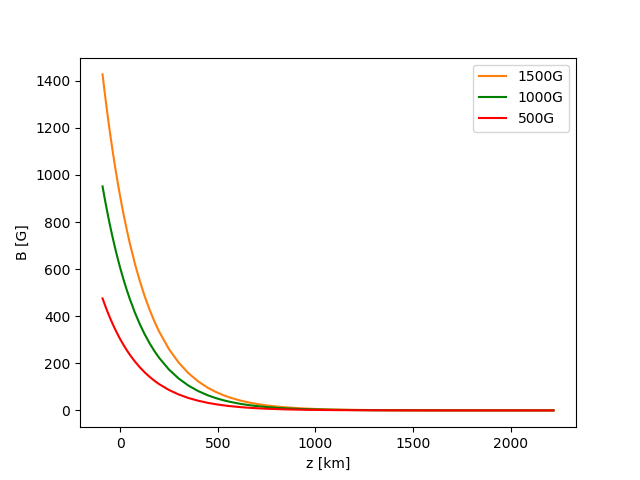
\includegraphics[scale=1]{fe_Campo_Magnetico}
\caption{ En esta gr\'afica se describe el comportamiento de la intensidad del campo magn\'etico. }
\label{fe_Campo_Magnetico}
\end{figure}

\begin{figure}[h]
\centering
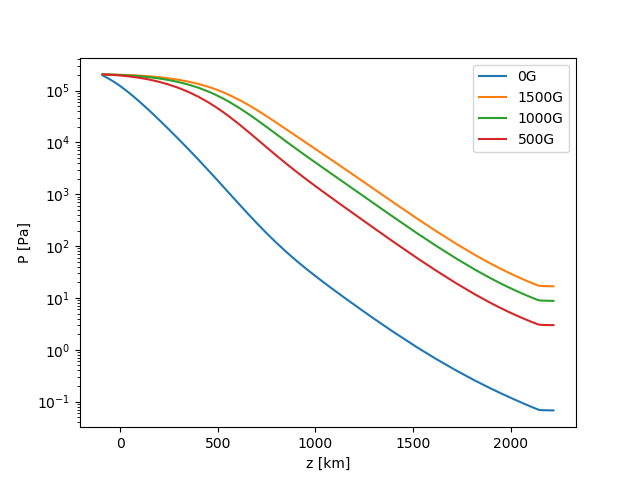
\includegraphics[scale=1]{fe_Presion}
\caption{ Aqu\'i se presentan cada una de las salidas de las simulaciones con los distintos valores de campo magn\'etico seg\'un los resultados anteriores.}
\end{figure}

\begin{figure}[h]
\centering
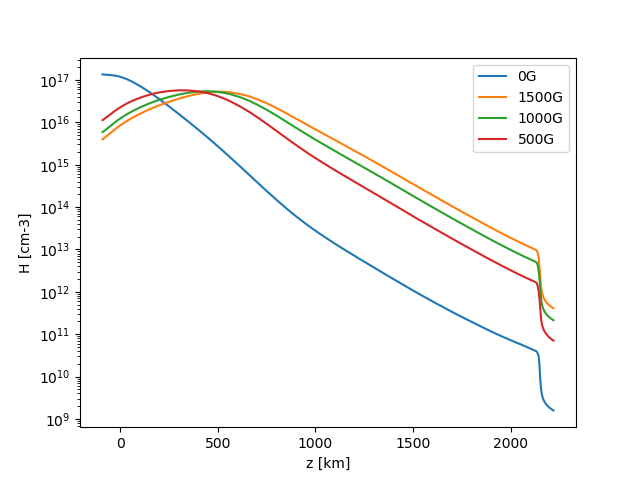
\includegraphics[scale=1]{fe_perfil_de_densidades}
\caption{ En esta figura se grafican el perfil de densidades de hidr\'ogeno.}
\label{am_perfil_de_densidades}
\label{fe_perfil_de_densidades}
\end{figure}

\begin{figure}[h]
\centering
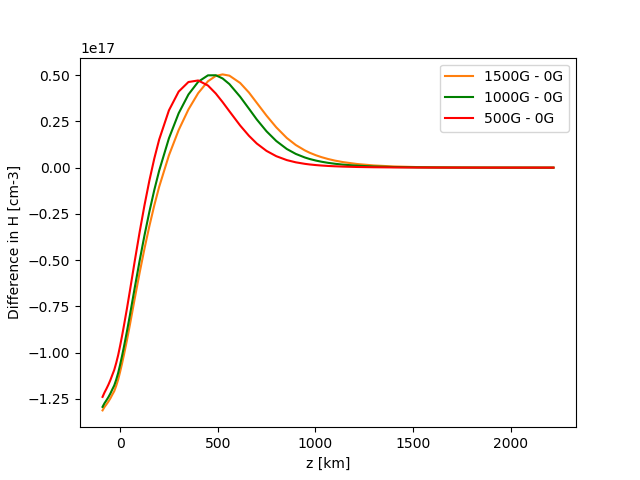
\includegraphics[scale=1]{fe_diferencias_absolutas}
\caption{ Aqu\'i se muestra una comparaci\'on entre las diferentes salidas de las densidades del programa.}
\label{fe_diferencias_absolutas}
\end{figure}

\begin{figure}[h]
\centering
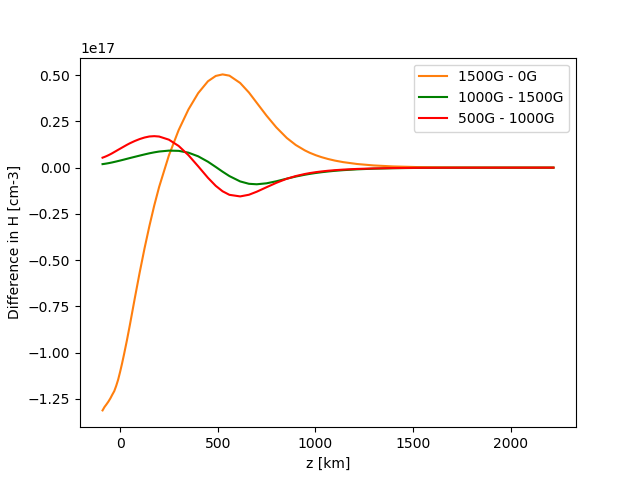
\includegraphics[scale=1]{fe_diferencias_relativas}
\caption{ Aqu\'i se muestra un diferencial de cada uno de las salidas de las simulaciones contra las salidas de la simulaci\'on con un valor m\'as bajo.}
\label{am_diferencias_relativas}
\label{fe_diferencias_relativas}
\end{figure}
\clearpage


\chapter{Discusi\'on y conclusiones}
Comparaci\'on entre ambos modelos, discusion y resultados

aproximaci\'on te\'orica
 



Springer Science \& Business Media, Aug 26, 2006

\begin{thebibliography}{9}

\bibitem{carrington} 
Robert D. Loper
\textit{Carrington-class events as a great filter for electronic civilizations in the drake equation} 
Astronomical Society of the Pacific, 2019.

\bibitem{VAULT1} 
A. Vourlidas, B. Sanchez, E. Landi, et al.
\textit{The structure and Dynamics of the Upper Chromosphere and Lower Transition Region as Revealed by the Subarcsecond VAULT Observations, Astronomy and Astrophysics} 
Solar Physics, 2010.

\bibitem{VALC}
J. E. Vernazza, E. H. Avrett y R. Loeser
\textit{Structure of the Solar Chromosphere. III. Models of the EUV Brightness Components of the Quiet Sun} 
The Astrophysical Journal Supplement Series, 1981.

\bibitem{C7}
J. M. Fontenla, E. H. Avrett y R. Loeser
\textit{Energy Balance in the Solar Transition Region. I. Hydrostatic Thermal Models with Ambipolar Difussion} 
The Astrophysical Journal, 1990.

\bibitem{PAKAL}
V. de la Luz
\textit{Modelaci\'on Tridimensional de la Atm\'osfera Solar para el Estudio de su Emisi\'on en Radio} 
2011.

\bibitem{loops} 
Markus Aschwanden. 
\textit{Physics of the Solar Corona} 
Springer Science \& Business Media, 2006.

\bibitem{flujoemergente} 
Rees and Seemel.
\textit{Line Formation in an Unresolved Magnetic Element: A Test of the Centre of Gravity Method} 
Astronomy and Astrophysics, 1978

\bibitem{Jackson} 
A. Vourlidas, B. Sanchez, E. Landi, et al.
\textit{Classical Electrodynamics} 
John Wiley and Sons, 1962.

\bibitem{NASAweb} 
Hathaway, D.
\textit{Chromospheric Features} 
https://solarscience.msfc.nasa.gov/feature2.shtml, NASA, 2014.

\bibitem{chromotemp} 
Fleishman G and Melnikov V
\textit{Gyrosynchrotron emission from anisotropic electron distributions} 
The Astrophysical Journal, 2003

\bibitem{magneticflux} 
N. Meunier
\textit{Solar chromospheric emission and magnetic structures from plages to intranetwork: Contribution of the very quiet Sun} 
Astronomy and Astrophysics, 2018

\end{thebibliography}




\end{document} 